%Chapter 3

\renewcommand{\thechapter}{3}

\chapter{UMER Apparatus and Diagnostics}
\label{ch:apparatus}

\section{UMER Layout}

UMER is laid out as a 36-sided polygon, comprised of 18 modular $20^o$ sections. Each section houses 2 dipole magnets over $10^o$ pipe bends and 4 quadrupole magnets in a FODO (focusing-defocusing) arrangement.

\section{UMER Beams}


	\subsection{Generation and Detection of Low-Current Beam}
	
	
	%%%%%%%%%%%%%%%%%%%%%%%%%%%%%%%%%%%%%%%%%%%%%%%%%%%%%%%%%%%%%%%%%%%%%%%%%%%%%%%%%%%%%%%%%%%%%%%%%%%%%%%%%%%%%%%%%%%%%%%%
	% IPAC 2015
	%%%%%%%%%%%%%%%%%%%%%%%%%%%%%%%%%%%%%%%%%%%%%%%%%%%%%%%%%%%%%%%%%%%%%%%%%%%%%%%%%%%%%%%%%%%%%%%%%%%%%%%%%%%%%%%%%%%%%%%%

\begin{figure}
\begin{center}
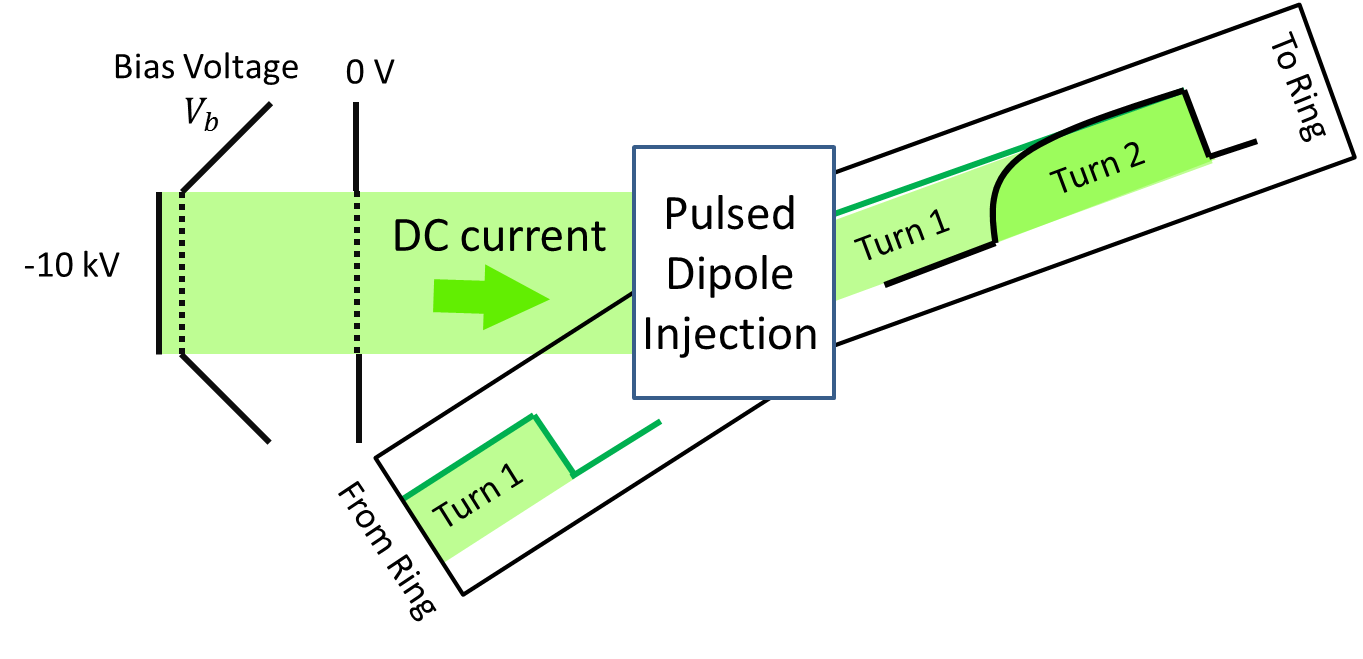
\includegraphics[width=\textwidth]{3.figures/DCbeam.png}
\end{center}
\renewcommand{\baselinestretch}{1}
\small\normalsize
\begin{quote}
\caption[]{Generation of variable current DC beam in UMER gun. Gate bias is lowered until DC current leaks through, pulse formation is done with injection dipole.}
\label{fig:DCbeamcartoon}
\end{quote}
\end{figure} 
\renewcommand{\baselinestretch}{2}
\small\normalsize
	
	
For experimental nonlinear dynamics, it is desirable to start with a primarily emittance dominated beam, with smaller space charge concentrations than the lower-limit UMER beam (0.6 mA, $\frac{\nu}{\nu_0}=0.85$), in order to isolate the space charge tune shift from the octupole tune shift. 
A nominally $50 \mu A$ beam was produced by reducing the cathode grid bias to allow leakage current and longitudinally gating the DC electron beam with the pulsed injector dipole. 
This resulted in a high-emittance, low current beam that maintained a DC signal for over 1000 turns, ultimately limited by the pulse length of the injection dipole. 
A low current, low emittance beam produced through photo-emission with a laser pulse is currently being explored as an additional UMER operating mode. 
%%%%%%%%%%%%%%%%%%%%%%%%%%%%%%%%%%%%%%%%%%%%%%%%%%%%%%%%%%%%%%%%%%%%%%%%%%%%%%%%%%%%%%%%%%%%%%%%%%%%%%%%%%%%%%%%%%%%%%%%
	
	

	
\section{Diagnostics}

\subsection{Beam Position Monitors}

\subsection{Wall Current Monitor}

\subsection{Transverse imaging}


\section{Measurement Techniques}

\section{Quadrupole as BPM technique} \label{sec:apparatus:quad-as-bpm}

First-turn position data is extrapolated from quadrupole response data, also called "quad as BPM" or "virtual BPM." A beam that is off-centered in a quadrupole will experience a dipole force acting on the centroid motion as well as a quadrupole focusing force that acts on the beam envelope, as shown in Fig. \ref{fig:simple-beamline}. The strength of the dipole kick will depend on the position of the centroid in the quadrupole as well as strength of the quadrupole. Variation of the quadrupole strength will cause variation of the centroid as detected on a downstream BPM. Knowledge of the centroid transformation between quadrupole and BPM allows reconstruction of the beam position. 

%%%%%%%%%%%%%%%% THEORY

\begin{figure}
\begin{center}
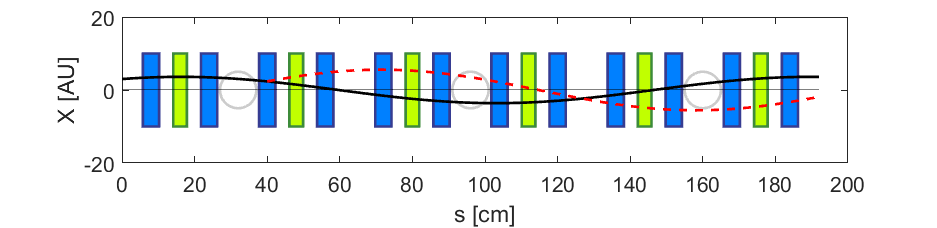
\includegraphics[width=\textwidth]{3.figures/quad-as-bpm/simple_beamline.png}
\end{center}
\renewcommand{\baselinestretch}{1}
\small\normalsize
\begin{quote}
\caption[]{Diagram of UMER beamline, with quadrupoles (blue), dipoles (green) and BPMs (circles). Black curve is possible centroid trajectory, dashed-red curve is perturbed centroid due to change in quadrupole strength at 40 cm. Phase advance per cell (32 cm) is $66.4^o$.}
\label{fig:simple-beamline}
\end{quote}
\end{figure} 
\renewcommand{\baselinestretch}{2}
\small\normalsize




In a lattice with low phase advance per cell (such as UMER, with $66.4 ^o$ and $67.5 ^o$ in the x,y planes), the particle motion is approximately sinusoidal, described by: 

\begin{equation} x(s) = A_1\cos{\frac{\sigma}{L}s} + A_2\sin{\frac{\sigma}{L}s}\end{equation}

The derivative of this motion is

\begin{equation} x'(s) = \frac{dX}{ds} = -A_1\frac{\sigma}{L}\sin{\frac{\sigma}{L}s} + A_2\frac{\sigma}{L}\cos{\frac{\sigma}{L}s}\end{equation}

Generally, the centroid is not confined to the reference orbit (the orbit that goes through the center of every quad), so the equilibrium centroid orbit oscillates with a frequency of $2\pi \times \nu$, with amplitudes $A$. Now, let's consider an orbit that has been perturbed, due to changing the strength of a single quad. We treat the quadrupole as "thin," an appropriate simplification when phase advance is low. Using the analog of thin lens optics in the paraxial approximation, $\Delta x' \approx tan \Delta x' = \frac{x_Q}{f}$ where $x_Q$ is the centroid offset in the quad and $f$ is the focal length. For a thin quadrupole, $\frac{1}{f} = \frac{G}{B\rho}$ for integrated gradient $G$ and magnetic rigidity $B\rho$. For UMER ring quadrupoles, $G=13.50I$ [Gauss/A] and for 10 keV electrons, $B\rho = 338.85$ G-cm. 

Consider a perturbed orbit $\tilde{x}(s) = x(s) + \delta x(s)$, where $s=0$ is the perturbed quad location. The initial conditions are $\tilde{x}(0) = x(0)$ and $\tilde{x'}(0) = x'(0) + \Delta x'_Q$ where $\Delta x'_Q = x(\frac{G \Delta I}{B\rho})$ is the change in angle due to perturbation on the quad. Letting $\delta x(s) = B_1\cos{\sigma s / L} + B_2\sin{\sigma s / L}$ and applying these initial conditions, we find $B_1 = 0$, $B_2 = x_Q L/\sigma \times G \Delta I / B\rho$ and the perturbed orbit is:

\begin{equation} \tilde{x}(s) = x(s) + x_Q \frac{L}{\sigma} \frac{G \Delta I}{B\rho} \sin{\frac{\sigma}{L}s} \end{equation}

With variation of the quadrupole strength, we find the dependence of the centroid position in a downstream BPM is linear in the position in the quadrupole, $x_Q$: 

\begin{equation} \frac{d \tilde{x}(s_{BPM})}{d\Delta I} = x_Q \frac{L}{\sigma} \frac{G}{B\rho} \sin{\frac{\sigma}{L}s_{BPM}} \label{eq:quad-response} \end{equation}

In the approach described here, we recover the first-turn position in the quadrupoles by measuring the slope $\frac{d \tilde{x}(s_{BPM})}{d\Delta I}$. A model of the ring using the VRUMER beam tracking code is used to calculate the constant $\frac{L}{\sigma} \frac{G}{B\rho} \sin{\frac{\sigma}{L}s_{BPM}}$, the result is a measurement of $x_Q$.
This is an essentially identical method to that described by Kamal Poor Rezaei \cite{KPRnote:2012}, 
with the main difference being the use of the VRUMER beam tracking code to calibrate position, rather than a transfer matrix calculation.  

VRUMER, described in detail in Appendix [TBD], is a simple orbit integrator written in Matlab, originally developed by Irving Haber to model transverse beam centroid behavior and test UMER-specific steering algorithms.
The model used here includes the measured background earth field, applied as a continuously acting, lab-frame-position dependent force based on linear interpolation between measurement points at the 36 dipoles.
This model does not include centroid kicks as a result of magnet fringe fields or the steering effect of the offset YQ magnet, although the framework can support these refinements.

At an operating point of 1.826 A, the UMER 6 mA beam has $\nu_x = 6.636$, $\nu_y=6.752$ \cite{RKnote:2010}. This corresponds to betatron wavelengths $\lambda_x = 1.736$ m, $\lambda_y=1.706$ m.
In the VRUMER simulation, horizontal and vertical tunes are equal (no edge focusing), $\nu=6.293$, equivalently $\lambda = 1.83$ m.
In this case, quadrupole strength parameters were set according to standard hard-edged approximation for the UMER quadrupoles: length$=4.475$ cm, peak strength $g=3.609$ G/cm, hard-edge factor $f=0.8354$.


\subsection{Systematic Error in Quad-as-BPM Calibration} \label{sec:steering:errors}

The previous section begs the question, what is the amount of systematic error introduced by differences between reality and the model used for calibration (in this case, VRUMER). Most notably, bare tune in the model and measured tune differ by $\Delta \nu_x = 0.340$ horizontally, $\Delta \nu_y = 0.459$ vertically. It is covenient to define phase advance per cell, $\sigma = \frac{2\pi\nu}{36}$. Additionally, there are measurement errors included in the measurement of position with BPM.

Examining the formula for $x_Q$ from Eq. \ref{eq:quad-response} above, re-written here as:

\begin{equation} x_Q = \frac{\sigma}{L} \frac{d \tilde{x}_{BPM}}{d \Delta I} \sin^{-1} \frac{\sigma}{L}s_{BPM} \end{equation}


Applying error analysis and assuming no significant error is introduced by our choice of $L$, $G$, $B\rho$, or $s_{BPM}$ in the model, we find the position error to be dependent on errors in the measured slope $m$, $\sigma_m$, and the systematic error of the model phase advance $\sigma$, $\sigma_\sigma$. 

\begin{equation} \frac{\sigma_{x_Q}}{x_Q} = \bigg[1-\frac{s_{BPM}}{L}\cot{\frac{\sigma}{L}s_{BPM}} \bigg]\frac{\sigma_\sigma}{\sigma} + \frac{\sigma_m}{m} 
\label{eq:quad-as-bpm-error}
\end{equation}

In this case, error $\sigma_m$ encompasses to statistical and systematic noise, as well as systematic calibration errors, related to the collection and processing of BPM data. For all the data shown here, $\sigma_m$ was taken to be the $90\%$ confidence bounds of the slope for the linear fit to the measured BPM position versus quadrupole strength curve. This encompasses shot-to-shot noise and nonlinearities introduced by beam scraping. Additionally, background was subtracted from scope traces to reduce the effect of systematic, repeatable noise picked up by the BPM amplifiers. 

$\sigma_\sigma$ is an error introduced by using the VRUMER model to calibrate quadrupole response data, and can be reduced by tweaking the focusing strength in the model. 

Fig. \ref{fig:quad-as-bpm-error} shows the dependence of the fractional error of measured position in the quadrupole, $x_Q$, as a function of separation between quadrupole and BPM used to measure quadrupole response. In this case, $\sigma_\sigma$ is taken to be the systematic error in phase advance between the VRUMER model and UMER experiment, $\sigma_\sigma = \mid \sigma_{sim} - \sigma_{exp} \mid = 0.06$. Only 8 discrete quad-BPM separations exist, in the range $[8,24,40,... 120]$ cm.


\begin{figure}
\begin{center}
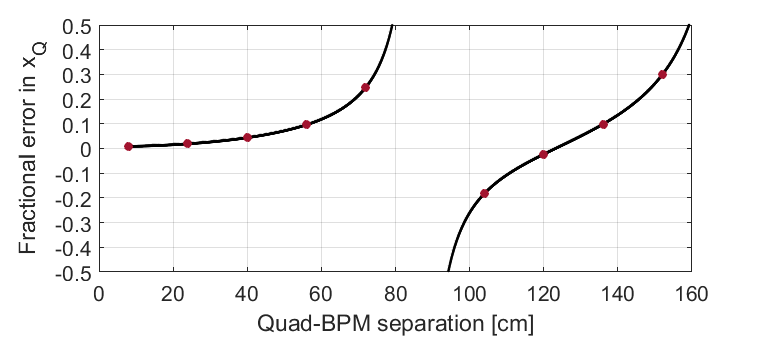
\includegraphics[width=\textwidth]{3.figures/quad-as-bpm/quad_as_BPM_error.png}
\end{center}
\renewcommand{\baselinestretch}{1}
\small\normalsize
\begin{quote}
\caption[]{Fractional error in quad-as-BPM position due to phase error, versus quad and BPM separation}
\label{fig:quad-as-bpm-error}
\end{quote}
\end{figure} 
\renewcommand{\baselinestretch}{2}
\small\normalsize


As seen from Eq. \ref{eq:quad-as-bpm-error}, the error approaches $\infty$ where $\frac{\sigma}{L}s_{BPM} = n\pi$. This is the point where the betatron wavelength is equal to the quad-BPM separation, a null point of the perturbed orbit $\delta x(s) = x_Q \frac{L}{\sigma} \frac{G \Delta I}{B\rho} \sin{\frac{\sigma}{L}s}$. Near this null, the returned quad-as-BPM measurement will have large errors, and in general be very sensitive to error in the BPM measurement as well as differences in the model and experiment. 


\begin{table}
\centering
\caption{"Next-downstream" Quad-BPM pairs with separations near half of a betatron wavelength, which results in large errors in the quad-as-BPM method.}
\label{tab:nulls}
\begin{tabular}{|c|c|}
Quad \# & Nearest BPM  \\
\hline
QR14 & RC5  \\
QR38 & RC11  \\
QR62 & RC17  \\
QR70 & RC1 (turn 2)  \\
\end{tabular}
\end{table}


In standard UMER operation, the BPM spacing is 64 cm (see Fig. \ref{fig:simple-beamline}), and the associated error is maximum $10\%$. However, 4 BPM's are omitted for injection, longitudinal focusing and the wall current monitor. Larger errors are permitted at larger separations. 
Table \ref{tab:nulls}) shows quadrupole-BPM pairs with fractional error $>1$. The spacing for these 4 pairs is 88 cm, close to half the betatron wavelength, $\frac{\lambda}{2} \approx 86 cm$. 

In subsequent data shown, the 4 quads identified in Table \ref{tab:nulls} use the response measured in the next downstream BPM in order to avoid artificial blow-up or suppression of measured $x_Q$ and $y_Q$.





\subsection{Tune Scans}	
	
	
\section{Lattice Configurations}
\subsection{FODO}

\begin{figure}[]
   \centering
   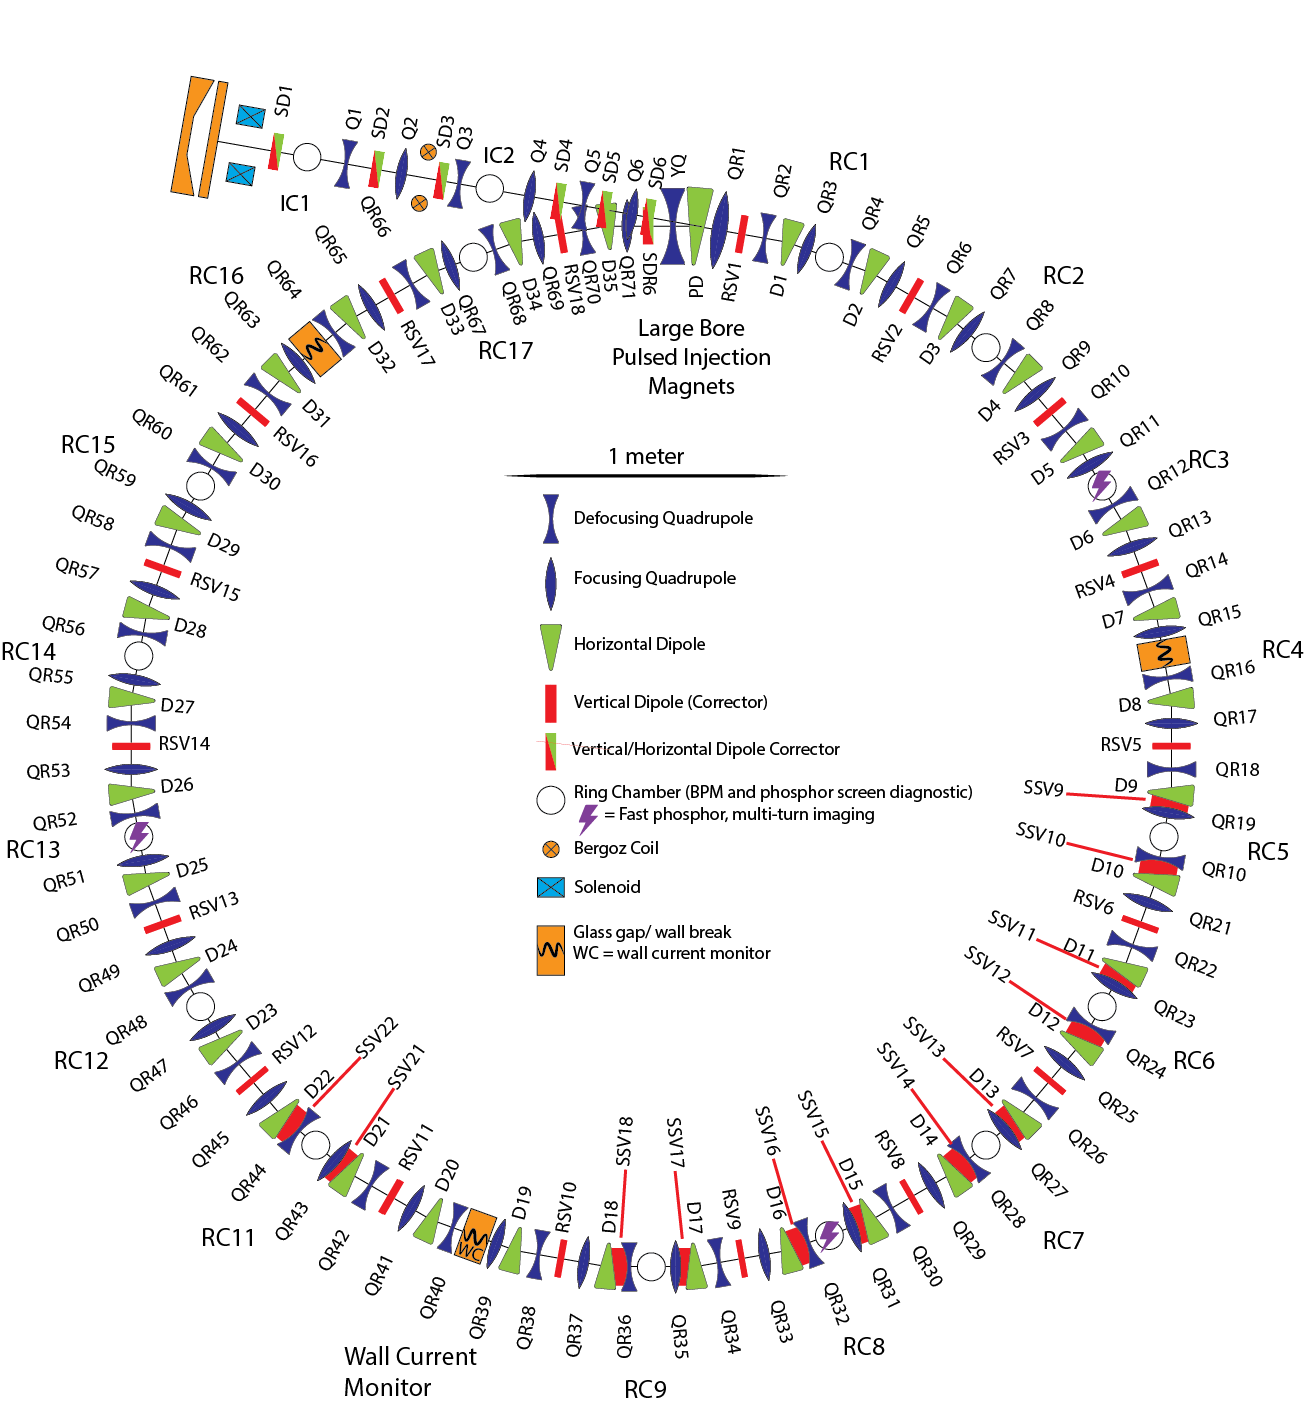
\includegraphics[width=\textwidth]{umer-diagram/full_ring.png}
   \caption{UMER ring, with all magnets labelled.}
   \label{fig:umerring}
\end{figure}

\subsection{Alternative FODO lattice}

\begin{figure}[]
%   \vspace*{-.5\baselineskip}
   \centering
   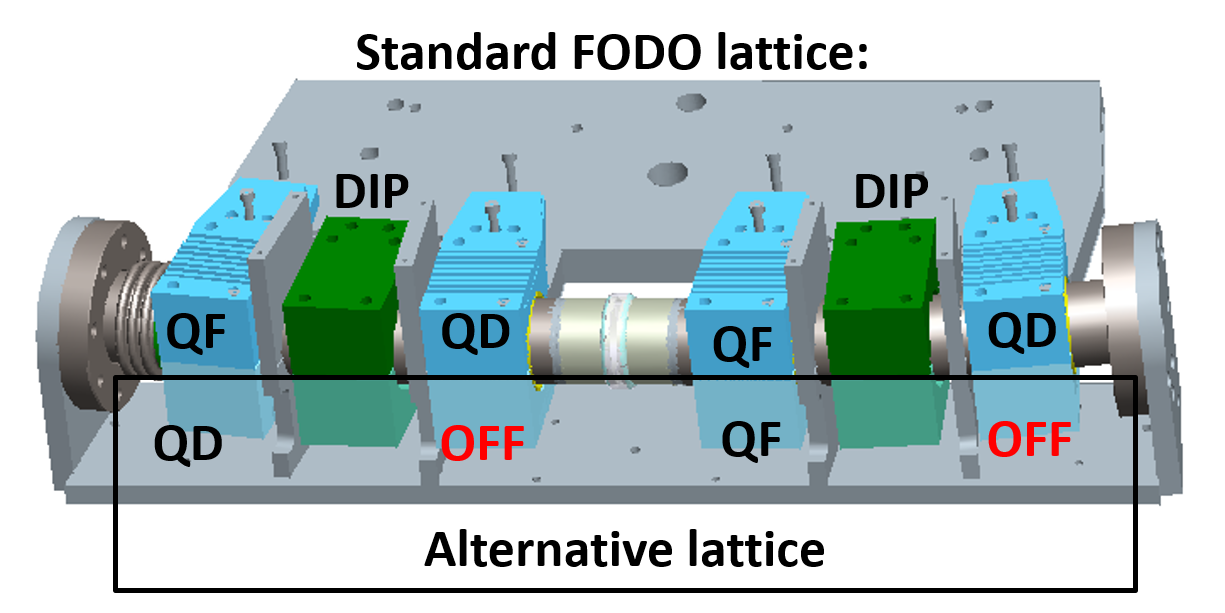
\includegraphics[width=0.7\textwidth]{3.figures/UMER_FODO.png}
   \caption{Two standard UMER FODO cells (blue quadrupoles and green dipoles). In the Alternatice lattice, the crossed quadrupoles are unpowered, leaving a vacancy for octupole elements.}
   \label{fig:FODOcell}
%   \vspace*{-\baselineskip}
\end{figure}

\begin{figure}[]
   \centering
   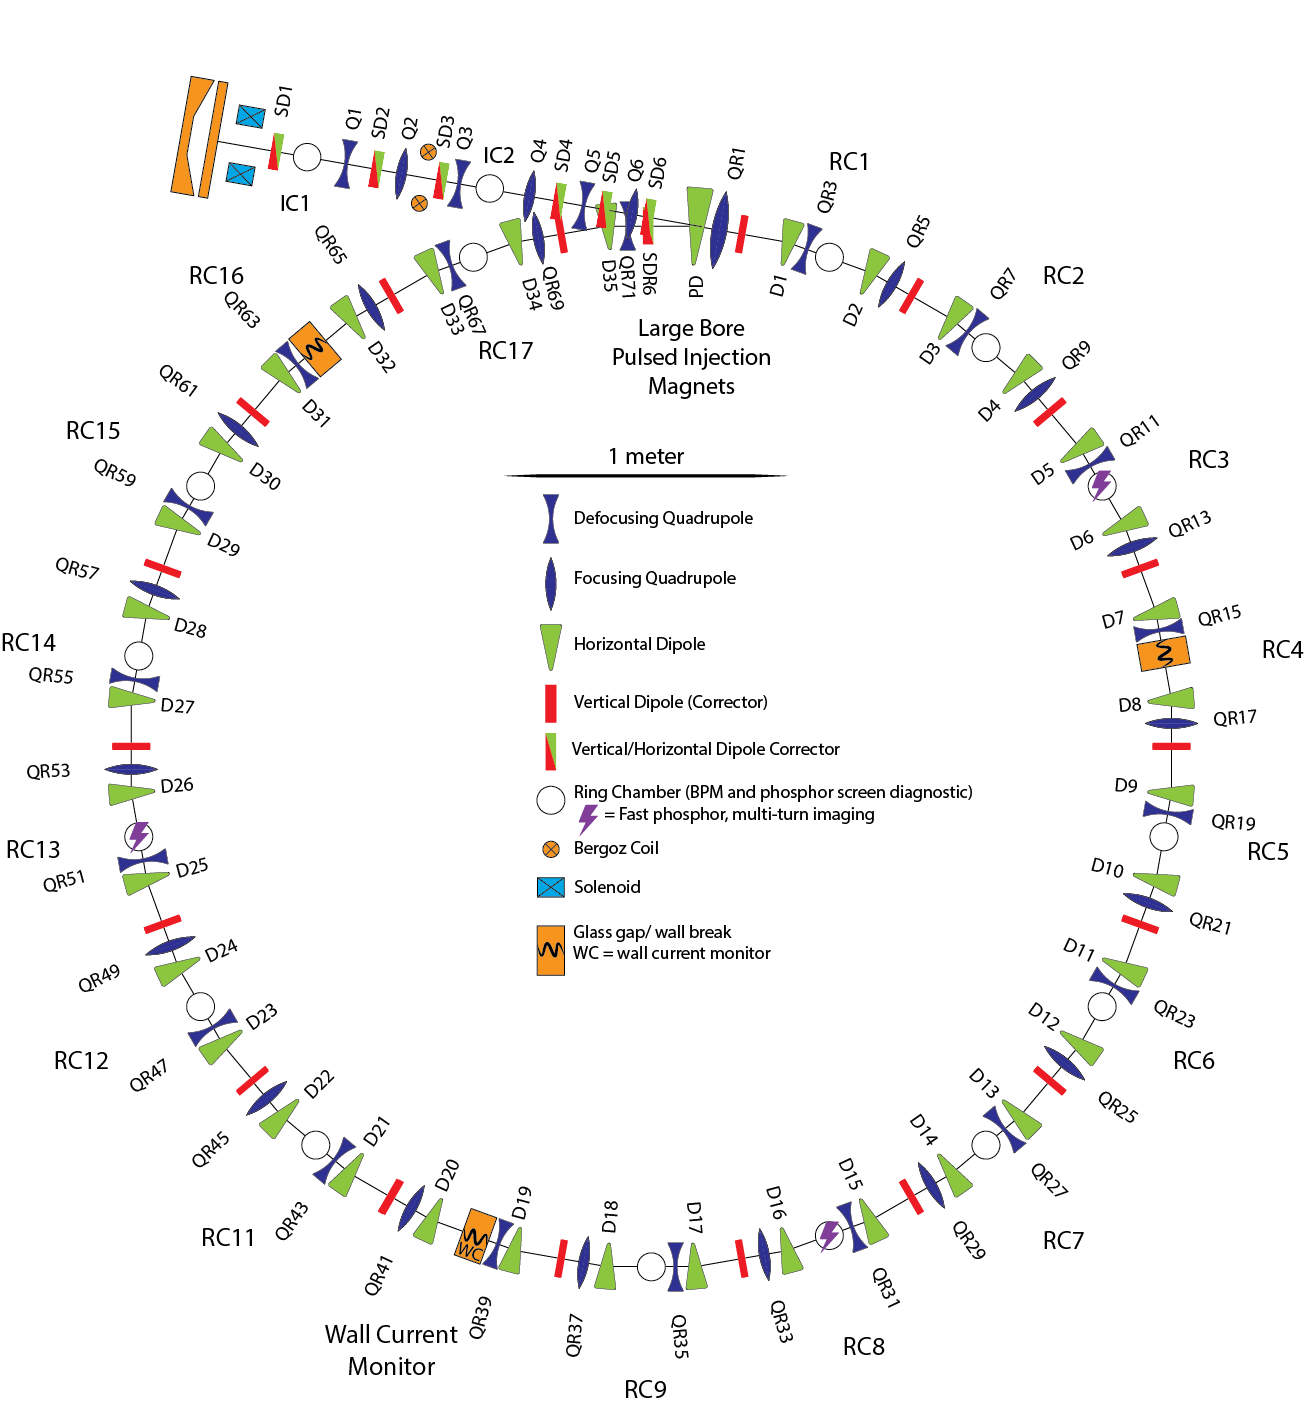
\includegraphics[width=\textwidth]{umer-diagram/altlat_full_ring.png}
   \caption{UMER ring in alternative lattice configuration.}
   \label{fig:altlatring}
\end{figure}

This configuration utilizes a mode of UMER operation known as the “alternative lattice” in which the total number of FODO cells in the ring is halved (by removing half of the quadrupoles).  The two lattices are illustrated in Fig. \ref{fig:FODOcell}. The nominal tune of the ring is also approximately halved, from $\nu \approx 6.7$ to $\approx 3.8$.






